\section{Resultados del modelado}
Esta sección presenta los resultados del entrenamiento de los tres modelos seleccionados sobre la vista minable Gold: Regresión Lineal, Árbol de Decisión Regresor y K-Means. Cada modelo se entrenó mediante un pipeline común de Spark MLlib (\texttt{VectorAssembler} $\rightarrow$ \texttt{StandardScaler} $\rightarrow$ algoritmo) y se evaluó utilizando los evaluadores estándar del paquete \texttt{pyspark.ml.evaluation}. Para los modelos supervisados se realizó un split aleatorio 80/20 con semilla fija (\texttt{seed=42}) sobre 6,502 observaciones municipio-año, lo que resulta en 5,217 filas para entrenamiento y 1,285 para test. Adicionalmente, se ejecutaron pruebas con diferentes combinaciones de hiperparámetros para cada modelo, requisito explícito del rúbrica.

\subsection{Regresión Lineal: grid de hiperparámetros}
La Regresión Lineal se entrenó con 12 combinaciones distintas de hiperparámetros, cruzando cuatro valores del parámetro de regularización (\texttt{regParam} en $\{0.0, 0.01, 0.1, 0.5\}$) con tres valores del parámetro de elasticidad (\texttt{elasticNetParam} en $\{0.0, 0.5, 1.0\}$, correspondientes a Ridge puro, ElasticNet balanceado y Lasso puro respectivamente).

\begin{table}[H]
\centering
\caption{Resultados de la regresión lineal sobre 12 combinaciones de hiperparámetros.}
\begin{tabular}{r r r r r}
\toprule
\textbf{regParam} & \textbf{elasticNet} & \textbf{TRAIN $R^2$} & \textbf{TEST $R^2$} & \textbf{TEST RMSE} \\
\midrule
0.000 & 0.00 & 0.4170 & 0.4070 & 16.27 \\
0.000 & 0.50 & 0.4170 & 0.4070 & 16.27 \\
0.000 & 1.00 & 0.4170 & 0.4070 & 16.27 \\
0.010 & 0.00 & 0.4170 & 0.4069 & 16.27 \\
0.010 & 0.50 & 0.4170 & 0.4068 & 16.27 \\
0.010 & 1.00 & 0.4170 & 0.4068 & 16.27 \\
0.100 & 0.00 & 0.4169 & 0.4067 & 16.28 \\
0.100 & 0.50 & 0.4168 & 0.4061 & 16.28 \\
0.100 & 1.00 & 0.4166 & 0.4053 & 16.30 \\
0.500 & 0.00 & 0.4167 & 0.4054 & 16.29 \\
0.500 & 0.50 & 0.4143 & 0.4016 & 16.34 \\
0.500 & 1.00 & 0.4115 & 0.3982 & 16.39 \\
\bottomrule
\end{tabular}
\end{table}

El comportamiento del modelo es estable a través del grid: el $R^2$ de test se mantiene en un rango estrecho entre $0.398$ y $0.407$. La mejor combinación corresponde a la regresión sin regularización (\texttt{regParam} = $0$), lo que sugiere que el conjunto de features ya seleccionado y normalizado no presenta multicolinealidad severa que justifique penalizar los coeficientes. El modelo seleccionado como mejor logra un $R^2$ de test de $0.4070$ con un RMSE de $16.27$ puntos en el puntaje global.

\textbf{Coeficientes del modelo lineal seleccionado.} Los coeficientes interpretados sobre el espacio estandarizado entregan el siguiente ranking de impacto marginal sobre el puntaje global:

\begin{table}[H]
\centering
\caption{Coeficientes de la regresión lineal sobre las features estandarizadas.}
\begin{tabular}{l r}
\toprule
\textbf{Feature} & \textbf{Coeficiente $\beta$} \\
\midrule
idx\_privacion              & $-8.7597$ \\
pct\_internet\_icfes         & $+5.5768$ \\
pct\_rural\_sisben           & $+3.1093$ \\
accesos\_per\_capita\_5\_16  & $+2.4697$ \\
POBLACION\_5\_16             & $+1.8583$ \\
n\_estudiantes               & $-1.6464$ \\
COBERTURA\_NETA              & $+1.6303$ \\
DESERCION                    & $-1.6148$ \\
APROBACION                   & $+0.9125$ \\
n\_proveedores               & $+0.6714$ \\
avg\_velocidad\_bajada       & $+0.2066$ \\
pct\_grupo\_A                & $-0.0586$ \\
\bottomrule
\end{tabular}
\end{table}

El intercepto del modelo es de $240.66$ puntos, que corresponde aproximadamente al puntaje promedio nacional. El coeficiente más fuerte en magnitud es el del índice de privación ($-8.76$): por cada incremento de una desviación estándar en la privación, el puntaje del municipio cae casi 9 puntos. El segundo coeficiente más fuerte es el de penetración de internet ($+5.58$), confirmando el peso de la conectividad. Otros coeficientes destacables incluyen \texttt{pct\_rural\_sisben} y \texttt{accesos\_per\_capita\_5\_16}, ambos positivos, lo que sugiere efectos compensatorios interesantes en municipios rurales con buena cobertura digital.

\subsection{Árbol de Decisión Regresor: grid de hiperparámetros}
El Árbol de Decisión se entrenó con 15 combinaciones distintas, cruzando cinco valores de profundidad máxima (\texttt{maxDepth} en $\{3, 5, 8, 10, 15\}$) con tres valores del número mínimo de instancias por nodo (\texttt{minInstancesPerNode} en $\{1, 5, 10\}$).

\begin{table}[H]
\centering
\caption{Resultados del Árbol de Decisión sobre 15 combinaciones de hiperparámetros.}
\begin{tabular}{r r r r r}
\toprule
\textbf{maxDepth} & \textbf{minInst} & \textbf{TRAIN $R^2$} & \textbf{TEST $R^2$} & \textbf{TEST RMSE} \\
\midrule
 3 &  1 & 0.3982 & 0.3837 & 16.59 \\
 3 &  5 & 0.3982 & 0.3837 & 16.59 \\
 3 & 10 & 0.3982 & 0.3837 & 16.59 \\
 5 &  1 & 0.4912 & 0.4735 & 15.33 \\
 5 &  5 & 0.4854 & 0.4686 & 15.40 \\
 5 & 10 & 0.4813 & 0.4794 & 15.25 \\
 8 &  1 & 0.6229 & 0.5104 & 14.79 \\
 8 &  5 & 0.6045 & 0.5115 & 14.77 \\
 8 & 10 & \textbf{0.5857} & \textbf{0.5214} & \textbf{14.62} \\
10 &  1 & 0.7146 & 0.4542 & 15.61 \\
10 &  5 & 0.6709 & 0.5004 & 14.94 \\
10 & 10 & 0.6350 & 0.5107 & 14.78 \\
15 &  1 & 0.8985 & 0.3671 & 16.81 \\
15 &  5 & 0.7943 & 0.4678 & 15.41 \\
15 & 10 & 0.7094 & 0.4968 & 14.99 \\
\bottomrule
\end{tabular}
\end{table}

El grid del árbol muestra un patrón clásico de \textit{overfitting} cuando se incrementa la profundidad sin restringir el tamaño mínimo de los nodos: con \texttt{maxDepth} = $15$ y \texttt{minInst} = $1$ el modelo alcanza un $R^2$ de entrenamiento muy alto ($0.8985$) pero un $R^2$ de test mediocre ($0.3671$), evidencia de que el árbol está memorizando ruido en lugar de aprender patrones generalizables. El mejor balance se obtiene con \texttt{maxDepth} = $8$ y \texttt{minInst} = $10$, configuración que logra un $R^2$ de test de $0.5214$ con un RMSE de $14.62$ puntos, superando claramente al mejor modelo lineal.

\textbf{Importancia de variables del árbol seleccionado.} El árbol entrega un ranking de importancia que complementa los coeficientes lineales.

\begin{table}[H]
\centering
\caption{Importancia de variables en el Árbol de Decisión seleccionado.}
\begin{tabular}{l r}
\toprule
\textbf{Feature} & \textbf{Importancia} \\
\midrule
idx\_privacion              & 0.4828 \\
pct\_internet\_icfes         & 0.2331 \\
pct\_rural\_sisben           & 0.0627 \\
POBLACION\_5\_16             & 0.0436 \\
pct\_grupo\_A                & 0.0433 \\
n\_estudiantes               & 0.0378 \\
accesos\_per\_capita\_5\_16  & 0.0336 \\
DESERCION                    & 0.0201 \\
COBERTURA\_NETA              & 0.0161 \\
APROBACION                   & 0.0116 \\
n\_proveedores               & 0.0080 \\
avg\_velocidad\_bajada       & 0.0074 \\
\bottomrule
\end{tabular}
\end{table}

El árbol confirma de manera contundente lo que la regresión lineal sugería: la privación multidimensional (índice $I1$ a $I15$ promediado) es por lejos la variable más explicativa del puntaje, con una importancia relativa del 48.3\%. La penetración de internet es la segunda variable más relevante, con un 23.3\%. Las demás features aportan individualmente menos del 7\%, lo que indica que el modelo se sostiene principalmente sobre dos factores: pobreza y conectividad.

\subsection{Comparativa final de modelos supervisados}
\begin{table}[H]
\centering
\caption{Comparativa final de los modelos supervisados sobre el conjunto de test.}
\begin{tabular}{l r r r r}
\toprule
\textbf{Modelo} & \textbf{TRAIN $R^2$} & \textbf{TEST $R^2$} & \textbf{TEST MAE} & \textbf{TEST RMSE} \\
\midrule
Regresión Lineal (default)       & 0.4169 & 0.4067 & 12.31 & 16.28 \\
Decision Tree (default)          & 0.6709 & 0.5004 & 11.21 & 14.94 \\
LR mejor del grid                & ---    & 0.4070 & ---   & 16.27 \\
\textbf{DT mejor del grid}       & \textbf{0.5857} & \textbf{0.5214} & ---  & \textbf{14.62} \\
\bottomrule
\end{tabular}
\end{table}

El árbol de decisión supera consistentemente a la regresión lineal en términos de capacidad predictiva sobre el test set, lo que se atribuye a su habilidad de capturar interacciones no lineales que el modelo lineal no puede expresar. Sin embargo, la regresión lineal mantiene su valor como herramienta de interpretación, dado que sus coeficientes son directamente leíbles como impacto marginal de cada variable. Ambos modelos son persistidos en HDFS (\texttt{/usr/proyecto/models/lr\_punt\_global} y \texttt{/usr/proyecto/models/dt\_punt\_global}) para inferencia futura.

\subsection{K-Means: selección del número de clusters}
Para el modelado no supervisado se aplicó K-Means sobre la vista minera filtrada al año más reciente disponible (2022) con un total de 1,098 municipios. Se probaron siete valores de $k$ y se evaluaron mediante dos métricas estándar: la suma de cuadrados dentro de los clusters (WCSS, \texttt{m.summary.trainingCost}) para el método del codo, y el coeficiente de silueta (\texttt{ClusteringEvaluator}) para la calidad de la separación.

\begin{table}[H]
\centering
\caption{Resultados del grid de K-Means para selección del número óptimo de clusters.}
\begin{tabular}{r r r}
\toprule
\textbf{k} & \textbf{WCSS} & \textbf{Silueta} \\
\midrule
2 & 4,399.40 & \textbf{0.4493} \\
3 & 3,573.68 & 0.4113 \\
4 & 3,180.22 & 0.3183 \\
5 & 2,917.36 & 0.2979 \\
6 & 2,784.15 & 0.2866 \\
7 & 2,579.93 & 0.2721 \\
8 & 2,449.81 & 0.2650 \\
\bottomrule
\end{tabular}
\end{table}

El coeficiente de silueta alcanza su máximo en $k = 2$ con un valor de $0.4493$, que indica una separación moderadamente buena de los clusters (valores por encima de $0.5$ se consideran fuertes, entre $0.25$ y $0.5$ aceptables). El WCSS muestra el patrón esperado de decrecimiento monótono, sin un codo dramático que sugiera un número de clusters claramente diferenciado. Por consistencia con la métrica de silueta, se selecciona $k = 2$ como el número de clusters final.

\begin{figure}[H]
\centering
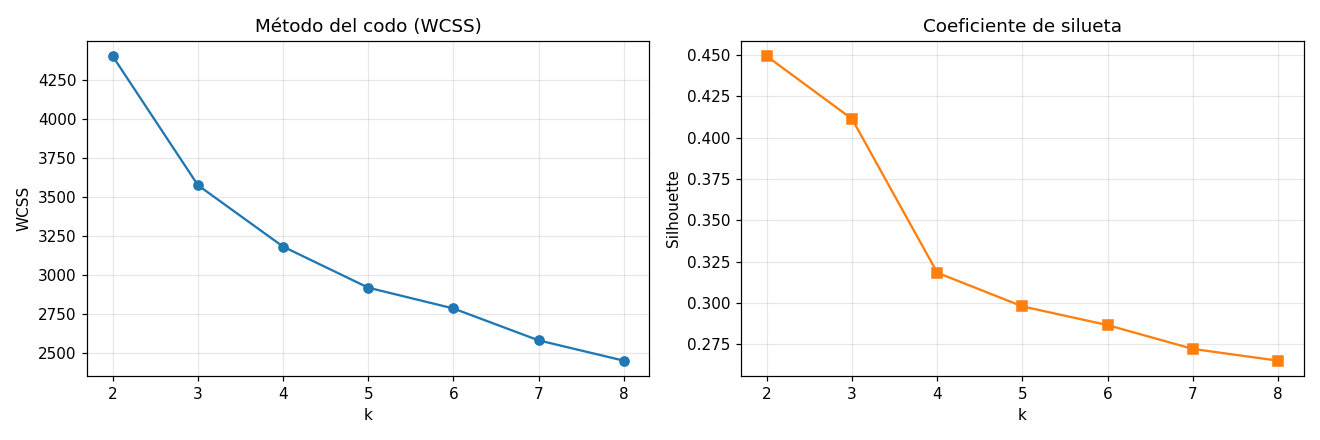
\includegraphics[width=0.95\textwidth]{figures/kmeans_eleccion_k.png}
\caption{Curvas de WCSS (método del codo) y coeficiente de silueta en función del número de clusters $k$.}
\end{figure}

\subsection{K-Means: perfilado de clusters}
Con $k = 2$ los 1,098 municipios se distribuyen en dos grupos claramente diferenciados.

\begin{table}[H]
\centering
\caption{Perfil promedio de cada cluster (valores en escala original).}
\begin{tabular}{c r r r r r r r}
\toprule
\textbf{Cluster} & \textbf{N° mpio} & \textbf{Punt.} & \textbf{\% Internet} & \textbf{Accesos pc} & \textbf{Idx. priv.} & \textbf{\% Grupo A} & \textbf{Cob. neta} \\
\midrule
0 & 603 & 227.6 & 38.6 & 0.528 & 4.39 & 48.8 & 82.8 \\
1 & 495 & 251.4 & 64.2 & 2.303 & 3.23 & 25.8 & 90.3 \\
\bottomrule
\end{tabular}
\end{table}

La interpretación de negocio de los dos clusters es directa. El \textbf{Cluster 0} agrupa 603 municipios con perfil de \textit{alta vulnerabilidad}: puntaje promedio bajo ($227.6$), baja penetración de internet ($38.6$\%), alta privación multidimensional ($4.39$ sobre 15), casi la mitad de la población en el grupo A del Sisbén ($48.8$\%) y cobertura neta promedio inferior ($82.8$\%). El \textbf{Cluster 1} agrupa 495 municipios con perfil de \textit{baja vulnerabilidad}: mejor puntaje ($251.4$), mucha mejor conectividad ($64.2$\%), menor privación ($3.23$) y mayor cobertura ($90.3$\%).

La diferencia de puntaje promedio entre los dos clusters es de aproximadamente 24 puntos, lo que coincide con la magnitud observada en la pregunta Q4 del análisis exploratorio. La identificación de estos dos grupos permite al Ministerio de Educación tomar decisiones diferenciadas: el Cluster 0 constituye el grupo objetivo prioritario del plan de acción, donde la combinación de baja conectividad y alta privación demanda intervenciones integrales (no solo digitales).

\begin{figure}[H]
\centering
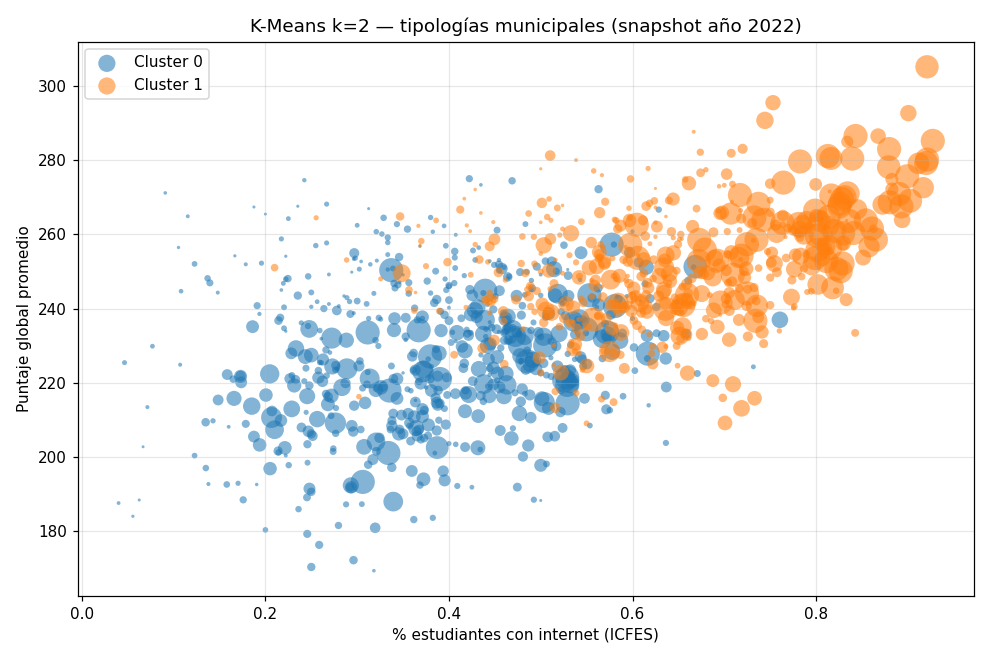
\includegraphics[width=0.95\textwidth]{figures/kmeans_clusters_scatter.png}
\caption{Distribución de los 1,098 municipios por porcentaje de internet en el hogar y puntaje global, coloreados por cluster K-Means.}
\end{figure}

\subsection{Persistencia de los modelos en HDFS}
Todos los modelos entrenados se persistieron en HDFS para garantizar reusabilidad e inferencia futura sin necesidad de reentrenar:

\begin{itemize}
    \item \texttt{/usr/proyecto/models/lr\_punt\_global}: Regresión Lineal con la mejor combinación del grid.
    \item \texttt{/usr/proyecto/models/dt\_punt\_global}: Árbol de Decisión con la mejor combinación del grid.
    \item \texttt{/usr/proyecto/models/kmeans\_k2}: K-Means final con $k = 2$.
\end{itemize}

La carga de cualquier modelo en una sesión futura se realiza con las clases correspondientes de \texttt{pyspark.ml}, lo que permite que el Ministerio o un equipo técnico puedan reutilizar los modelos sobre nuevos datos sin tener que volver a ejecutar el pipeline completo.
